\if0
1. Audio Watermarking in Recording Time
	ほぼ変更なし
2. Preliminary Study for Modulating Method
	透かし仕様確定の事前研究として、二種類の変調手法を比較した
	可聴域を用いた高速伝達手法であるAcoustic OFDM
	FSKを拡張したオリジナルの手法であるAcoustic DTMF
	結果、後者のほうが今回の目的には適することが判明した
3. Acoustic DTMF in Inaudable Frequency Range
4. Packet Structure
\fi

\chapter{Watermarking Scheme}

\section{Audio Watermarking in Recording Time}

% 既存の音声透かし手法は適用できない
To enable embedding annotations for audio/visual editing in audio data, we owe fundamental idea to convert a digital data into an acoustic representation to existing audio watermarking techniques.
However, some significant differences between basic audio watermarking and embedding annotation for editing support make it difficult to apply existing watermarking techniques straightforwardly to our purpose.

% ビデオ録画時に埋め込むので要請が異なる
In principle, the purpose of watermarking techniques is to add extra information like indication of intellectual property rights to existing contents by means of signal processing, therefore usually watermarking is conducted in the post-production stage.
On the other hand, our purpose requires embedding extra data in the audio track of a video during shooting it with a video camera to record annotations of a scene to support content creation.
For this reason, our recording-time watermarking has different technical requirements from basic audio watermarking techniques.

% 特殊なデバイスが使えない
Firstly, any requirements of extra equipment like special microphone and audio mixer are not desirable.
Because our purpose is to support creators to make audio/visual contents, we should minimize hardware constraints and allow users to use our annotating technique with their favorite equipment for making content such as high-resolution camera and hi-fi audio recording system.
% リアルタイム重畳が必要
Secondly, host signal cannot be modified to embed data in our recording-time watermarking because host signal and annotation data are recorded simultaneously, unlike ordinary watermarking techniques take an existing content as a host signal to apply signal analysis and some modification such as phase-shifting for embedding data. % ToDo: because節の論理が不明瞭かも
Recently some techniques called {\it real-time watermarking} have been presented. Though these techniques realize real-time embedding of watermarking in contents, these techniques are not suited for our purpose because they require extra equipment for digital signal processing.
% ToDo: referenceを付ける, 論文を詳しく読んで内容を検討する
% 耐攻撃性は不要
Thirdly, since our watermarks are used only in editing process, durability and transparency of watermarks is not very important, unlike ordinary watermarks are required to be hidden and resistant to elimination because most of them are embedded to contain essential information for preserving the content from abuses.
In contrast to ordinary watermarks, watermarks for editing support should be able to be eliminated completely after the editing process because they have no immediate value for consumers of contents.

% これらの条件から、host signalを書き換えられないので、加算的に合成することにした
% watermarkingに用いた周波数成分は上書きされて消えてしまうので、聴取に影響を与えないことが問題
From these preconditions, we decided to use modulated tones of certain frequency bands for watermarking, making watermarking process significantly simple as generating encoded tones from input data, transmitting them from a speaker near the microphone of a camera, and recording them as environmental sounds.
In this process, watermark signals and host signals are mixed in air like {\it sonic watermarking} by Tachibana. \cite{tachibana2003audio}
Removal of watermarks can also be simplified because eliminating certain frequency component from an audio signal can be done easily by applying a band elimination filter (BEF).
One problem is that, since certain frequency components of host signal would be overwritten by the watermark signals and also be eliminated in removing watermarks, we should decide frequency range to use not to spoil listening impressions.

% 前提条件
% ところで音声ファイルは44.1kHzで収録されるが、人は16kHzくらいまでしか聴こえない…
Most of common media formats use 44.1 kHz as their audio sampling rate, and virtually all video cameras and audio recorders can record sounds in this rate. It means that we can record media files that contain sounds with frequency up to 22.05 kHz with common equipment, since a discrete signal can contain sampled signals with frequencies lower than half of its sampling rate, according to the Nyquist-Shannon sampling theorem. \cite{shannon1949communication}
Human's hearing range is well-known to be between 20 Hz and 20 kHz, however some studies showed that absolute threshold of hearing (ATH) increases rapidly along with the frequency above 14 kHz and some people can not notice sounds above 18 kHz completely. \cite{:/content/asa/journal/jasa/86/4/10.1121/1.398698, ashihara2006hearing}
% in practice, sounds with frequencies higher than about 18000 Hz cannot noticed by ordinary people unless they are informed the appearance of sounds in advance.
Because of these facts, digital data can be recorded in an audio sequence almost imperceptibly to human with commons video cameras, if they are converted to audio signals with frequencies between about 18 kHz and 22 kHz.

% カメラに装着したスマートフォンをトランスミッタとして用いる
In our system named AnnoTone, annotation data are converted to inaudible modulated sounds in frequency band of 17600Hz to 20000Hz and transmitted to a microphone of a video camera from a speaker of a smartphone attached to the camera.
% GPSや加速度センサーをはじめとしたスマートフォンのセンサー群やタッチパネルUIの入力をアノテーションとして吹き込むことが出来る
A type of annotation data can vary depending on its usage, for example, values of various sensors carried on a smartphone such as GPS and accelerometer can be coded, and user inputs from user interfaces displayed on a touch panel of a smartphone are also available to make annotations.
% 異なるアノテーションは別々のアプリを用いて吹き込むが、透かし生成処理はライブラリ化されている
Different types of annotations are recorded using different smartphone applications, however core process of generating and extracting watermark signals is provided as a software library therefore many applications could use it for annotating.


\section{Preliminary Study for Modulating Method}

% ビットレートの要件 ... double*3を入れるには200bpsは必須
Considering practical usage of annotations for content editing, we thought that in minimum 200 bps is required as the payload rate of watermarking, because if an user wants to record a value of a sensor (e.g. GPS) consists of two or three double-precision floating-point number every seconds, 8 (bit/byte) * 8 (bytes) * 3 = 192 (bits) should be able to embedded in one second.
% ヘッダや透かし間ギャップを考慮すると400bpsは欲しい
Taking overhead from packet header and required gap between watermarks for stability of decoding into account, at least 400 bps is desirable as the gross bit rate of our watermarking technique.

% 非可聴域を用いて変調を行うに当たって、我々は予備調査を行った
We conducted a preliminary study to choose appropriate method for modulating digital data in inaudible frequency range that satisfies this requirement for bit rate.
In this study, we implemented watermark transmitters and demodulators for two modulation methods and roughly evaluated their performance by using them in real hardware setup.

% 一方はOFDM
The first method uses orthogonal frequency-division multiplexing (OFDM) to make full use of available bandwidth over 18 kHz, following the idea of Matsuoka's {\it Acoustic OFDM} \cite{matsuoka2008acoustic}.
% OFDMとは
OFDM is a specialized variety of frequency-division 
multiplexing (FDM) that uses multiple sub-carriers with different frequencies to transmit information in parallel.
A signal of OFDM is synthesized by composing signals of all sub-carrier waves.
% OFDMの特徴
In OFDM, carrier frequencies are selected in orthogonal, in other words, signals of sub-carriers are independent of and do not interfere each other.
This characteristic realize closer spaces between carrier frequencies and transmitting larger number of sub-carriers than ordinary FDM in certain bandwidth, therefore using OFDM increases bit rate of transmission.
% 用いた条件
In our preliminary study, eight sub-carriers with equally spaced frequencies between 17900 Hz and 20000 Hz were used to send octet bits in one signal, and each sub-carrier signal was modulated using differential binary phase shift keying (D-BPSK) in 100 bps (10 milliseconds per unit signal).
In total, gross bit rate was 800 bps in the condition, which satisfies the requirement mentioned above.

% 他方はDTMF
The other method also employs multiple sub-carriers with different frequencies to transmit information more than a bit in a signal, however it uses dual-tone multiple-frequency (DTMF) technique for multiplexing.
A tone of DTMF is a composition of just two sinusoidal waves of different frequencies, and combination of the two frequencies represents the value of the signal.
Since the number of possible tone varieties of $n$-frequency DTMF is $_n C _2$, at most $\log_2 {}_n C _2$ bits can be sent in a signal.
%In push-button telephone system, DTMF using eight frequencies is used to represent 16 characters per signal for communication between devices.
% DTMFの特徴
In DTMF, the amount of information can be sent in a signal is smaller than OFDM if the number of sub-carriers are same, however signal intensity of each frequency can be much stronger when that of composed signal is restricted by hardware constraints because only two sub-carriers are composed simultaneously.
% 用いた条件
In this study, we used seven sub-carriers with equally spaced frequencies between 17600 Hz and 20000 Hz for DTMF. Since $_7 C _2$ is 21, 16 combinations among all pairs of seven frequencies were used to represent four bits per signal.
The length of a signal was set 10 ms, the same as that of first method.
In total, gross bit rate was 400 bps in the condition.

% 実験結果
As the result of the study, we found the first method with OFDM not suited for our purpose because of its worse embedding performance besides its higher bit rate.
Extraction of watermarks is instable in the method due to the weaker intensity of each sub-carriers because of small output power of a speaker of a smartphone.
% 大きいスピーカーを使えば解決するが、今回の目的には適切ではない
However the embedding performance would be gained enough if a loud speaker with enough power could be available, using OFDM seemed not to be appropriate choice since small hardware constraint is required in our purpose.
% DTMFを使うことにした
In conclusion, we decided to use DTMF in our watermarking scheme appreciating its higher reliability.

% ToDo: それぞれのスペクトログラムの比較を入れる

%\section{Acoustic OFDM in Inaudible Frequency Range}
%% ビットレートの要件 ... double*3を入れるには200bpsは必須
Considering practical usage of annotations for content editing, we thought that in minimum 200 bps is required as the payload rate of watermarking, because if an user wants to record a value of a sensor (e.g. GPS) consists of two or three double-precision floating-point number every seconds, 8 (bit/byte) * 8 (bytes) * 3 = 192 (bits) should be able to embedded in one second.
% ヘッダや透かし間ギャップを考慮すると400bpsは欲しい
Taking overhead from packet header and required gap between watermarks for stability of decoding into account, at least 400 bps is desirable as the gross bit rate of our watermarking technique.

% 18kHz以上の帯域幅を有効に使うため、OFDMを採用した
To satisfy this requirement for bit rate, we adopt orthogonal frequency-division multiplexing (OFDM) as the modulation method to make full use of available bandwidth over 18 kHz, following the idea of Matsuoka's {\it Acoustic OFDM} \cite{matsuoka2008acoustic}.
% OFDMとは
OFDM is a specialized variety of frequency-division multiplexing (FDM) that uses a number of sub-carriers with different frequencies to transmit information in parallel.
In OFDM, carrier frequencies are selected in orthogonal, in other words, signals of sub-carriers are independent of and do not interfere each other.
This characteristics realize closer spaces between carrier frequencies and transmitting larger number of sub-carriers than ordinary FDM in certain bandwidth, therefore using OFDM increases bit rate of transmission.

% 17.9kHz~20khzの8並列で送ってる
AnnoTone uses 8 sub-carriers with equally spaced frequencies between 17900 Hz and 20000 Hz (17900 Hz, 18200 Hz, 18500 Hz, 18800 Hz, 19100 Hz, 19400 Hz, 19700 Hz, 20000 Hz) thus one byte can be sent in one parallel signal.
% サブキャリアのモジュレーションについて
Each sub-carrier signal is modulated using differential binary phase shift keying (D-BPSK) in 100 bps (10 milliseconds per unit signal).
D-BPSK represents binary data in a series of unit signals by phase shifting of certain frequency component.
A unit signal represents `` 1 '' when the phase of the signal is same as that of previous one, it represents `` 0 '' when the phase of the signal is shifted $\pi$ radians from that of previous one.
Using OFDM reduces computational cost of decoding significantly, enabling D-BPSK demodulation of each sub-carrier to be done in parallel without applying any filter such as band pass filter (BPF).
% 合計のビットレートは
In total, gross bit rate is 800 bps in our system, which satisfies the requirement mentioned above.


% 内容としては Packet Structure + DTMFのエンコード
\section{Acoustic DTMF in Inaudible Frequency Range} 
% DTMFに関して多少の詳細説明
A watermark of AnnoTone is modulated using DTMF technique mentioned above.
It can contain any kind of annotation data such as integer value, floating-point number, character string, and set of them.
Annotation data is serialized to a byte array and converted to a watermark packet structured as below.

% スペクトログラム
\begin{figure}[htbp]
 \begin{center}
  \includegraphics[width=120mm]{watermarking_spectrogram.png}
 \end{center}
 \caption{The signal spectrogram of a watermark packet that contains a geolocation data from GPS sensor.}
 \label{fig:watr_spec}
\end{figure}

% データフレームの定義
A data frame is the minimum unit of data representation in the watermarking scheme, and is a DTMF signal composed from two sinusoidal waves of the seven sub-carrier frequencies with length of 10 ms.
Since each data frame represents 4-bits information from 0 to 15, a data of one byte is encoded into two data frames.
The former frame represents the lower four bits and the latter represents the higher four bits of a byte.

% パケット模式図
\begin{figure}[htbp]
 \begin{center}
  \vspace{5mm}
  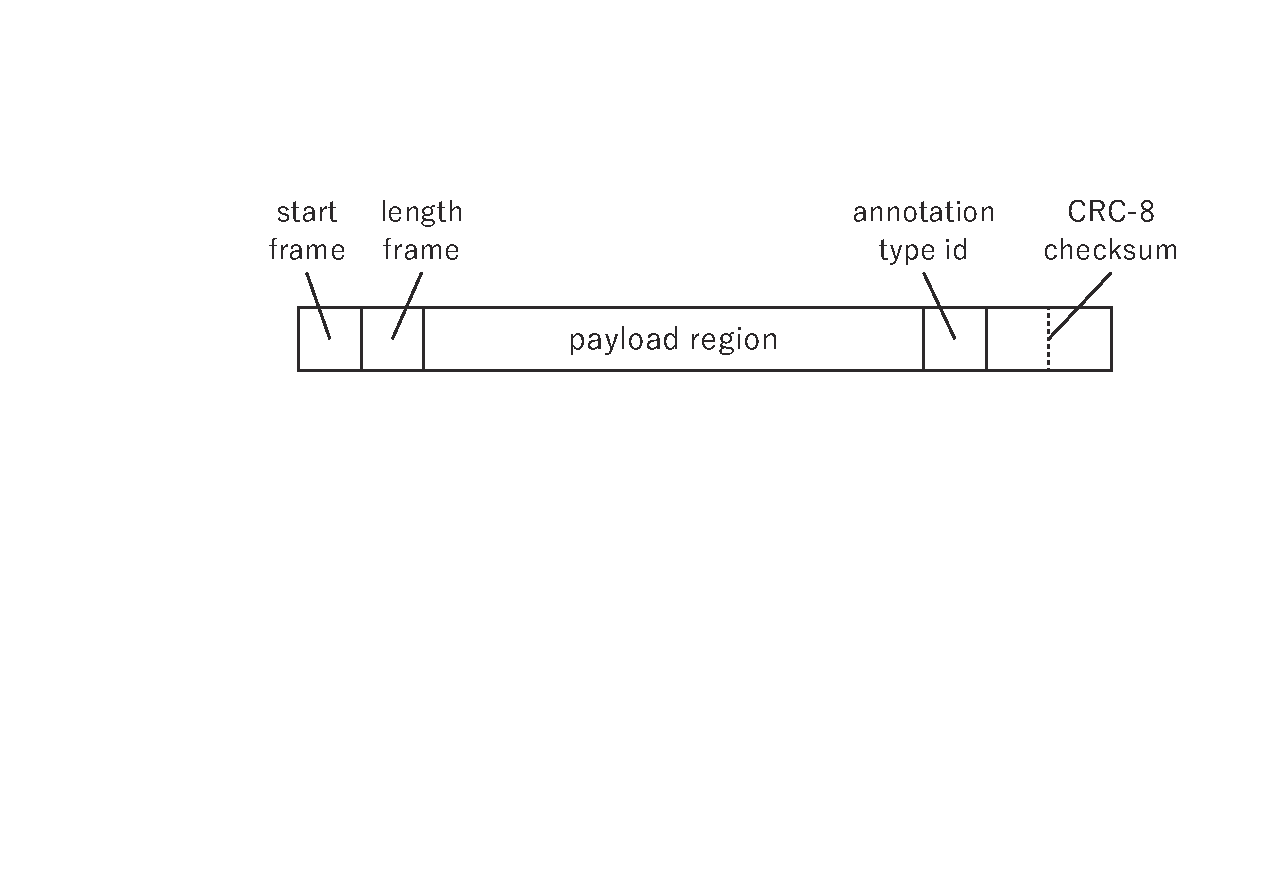
\includegraphics[width=120mm]{watermarking_packet.pdf}
 \end{center}
 \caption{Packet structure.}
 \label{fig:watr_pack}
\end{figure}

% パケットの定義
A packet is a set of several successive data frames representing an annotation data.
The data frame at the head of a packet is called start frame. It is fixed to represent ``2'', and it functions only as a sign of the start position of the packet. There is no special reason for choosing this number.
The second data frame specifies the length of payload region following it to be $ 2^n $ bytes where $n$ is the value of this data frame. It enables a payload size to vary depending on the type of an annotation. Consequently, the size of a packet can also vary.
From the third data frame, a payload region containing the body of an annotation data starts and continues for the length specified in the second data frame.
Multi-byte data such as integer values are ordered in little endian, and multiple data are arranged in their original order in a payload region.
For example, an array of two short integer values \{0x1234, 0x5678\} would be arranged in a payload region as \{4, 3, 2, 1, 8, 7, 6, 5\}.
The data frame after the end of a payload region represents the annotation type id from 0 to 15 to distinguish multiple kinds of annotations embedded in one media file.
An annotation type id for a watermark can be decided arbitrarily by annotating applications.
A packet ends with two data frames representing the CRC-8 checksum of the packet for error detection in decoding. The polynomial for calculating CRC-8 checksum is $x^8 + x^7 + x^6 + x^4 + x^2 + 1$.

